\section{Focusing the LMT}

\subsection{}
Like all telescopes, the LMT must be focused several times a night.
To do this we make a small map of a bright point-like source and then adjust the z-position of the secondary mirror until the point spread function (the telescope’s response function) is round and maximized. 

We are given 5 maps of a point source taken on February 7, 2015. Along with them, we are given 5 other fits files which are the corresponding weights, $(1/\sigma^2)$, of the point source maps. Each map corresponds to a different z-position of the secondary mirror as shown in Table \ref{tab:LMTmaps}

We can use the Levenberg-Marquardt (LM) method \footnote{lmfit python package} to fit the point source maps to a 2D Gaussian because a point source will look as a 2D Gaussian to the telescope. The LM method is a way to minimize the $\chi^2$ function.
% using a seamless transition from the steepest descent method (STM) and the inverse Hessian method (IHM).

The point source maps can be fitted to a 2D Gaussian described by the following equation
\begin{equation}
    f(x,y)=Ae^{-a(x-x_0)^2-b(x-x_0)(y-y_0)-c(y-y_0)^2}
\end{equation}
where 
\begin{align}
    a=\frac{\cos^2\theta}{2\sigma_x^2}+\frac{\sin^2\theta}{2\sigma_y^2},\\
    b=-\frac{\sin 2\theta}{2\sigma_x^2}+\frac{\sin 2\theta}{2\sigma_y^2},\\
    c=\frac{\sin^2\theta}{2\sigma_x^2}+\frac{\cos^2\theta}{2\sigma_y^2},
\end{align}
$A$ is the amplitude, $(x_0,y_0)$ is the center of the peak, $\sigma_x,\sigma_y$ are the width of the peak and $\theta$ is a rotation angle.

Using the lmfit package we can apply the LM method to find the parameters that minimize the $\chi^2$ function for the 2D Gaussian. To do so, we first define \emph{lmfit.Model()} to use the 2D Gaussian definition specifying the independent variables $x$ and $y$, and the parameters $A,x_0,y_0,\sigma_x,\sigma_y,$ and $\theta$. After defining the model, we use \emph{lmfit.Model.fit} to fit each of the maps using the weight maps and the initial estimate of all parameters. The result are the best values of the parameters that minimizes the $\chi^2$ function. 
Figure \ref{fig:lmtRaw} shows the raw maps, the fitted map using the best values of the parameters $A,x_0,y_0,\sigma_x,\sigma_y,$ and $\theta$ and a map of the residuals, $raw-fit$. 

Once we have the best fit parameters for each map, we extract the amplitude, $A$, from each map and plot it against the z-position of the secondary mirror. This set of data will be fitted to a quadratic model described by,
\begin{equation}
    f(z)=a_0+a_1z+a_2z^2
\end{equation}
where $z$ is the z-position of the secondary mirror as given in Table \ref{tab:LMTmaps}. 

Noting that the quadratic model is linear in its parameters, we choose to do the fit using the least squares method with SVD. From this fit, we obtained the maximum and select its corresponding z-position as the best position for the secondary mirror. Figure \ref{fig:lmtquadfit} shows the amplitude and z position of the secondary mirror alongside the least squares fit using SVD and the best z-position for the secondary mirror, which for this case is \SI{-0.57}{\milli\m}.

% The data is stored in the file maps.tar.gz on the class Moodle page. You can unpack that on a linux computer with the commands: gunzip maps.tar.gz and tar -xcv maps.tar. This will give you a set of 10 fits files (remember fits from homework 1) that you will read. The files with “signal” in the name are the maps of the source. The files with "weight" in the name are images with each pixel representing the weight $(1/\sigma^2)$ of each pixel in the corresponding signal map.

% Putting all this together, use the lmfit Levenberg-Marquardt fitting package to fit each image to a 2-d gaussian. 
% Find the best fit amplitude in each case and fit the best fit amplitudes to the function
% \begin{equation}
%     f(z)=a_0+a_1z+a_2z^2
% \end{equation}
% where z is the z-position of the secondary as given in the table below.

% Use the results of this
% fit to determine the best-fit position of the LMT's secondary mirror.

\begin{table}[h]
    \centering
    \begin{tabular}{|c|c|}
        \toprule
         Observation  & z-position (mm)  \\
         \midrule
         35114 & -3.0\\
         35115 & -2.0 \\
         35116 & -1.0 \\
         35117 & 0.0 \\
         35118 & 1.0\\
         \bottomrule
    \end{tabular}
    \caption{List of observation maps and their corresponding z-position of the secondary mirror of the LMT.}
    \label{tab:LMTmaps}
\end{table}

\begin{figure}
    \centering
    \begin{subfigure}[b]{.45\textwidth}
        \centering
        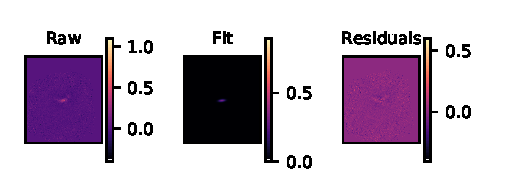
\includegraphics[height=100pt]{CodeAndFigures/DataFits4.pdf}
        \caption{Data:35114}
        \label{fig:lmtFit4}
    \end{subfigure}
    \begin{subfigure}[b]{.45\textwidth}
        \centering
        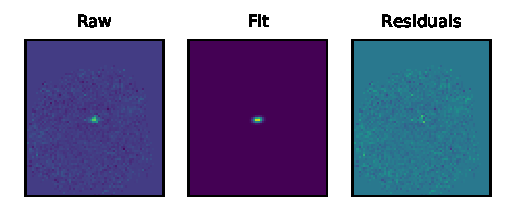
\includegraphics[height=100pt]{CodeAndFigures/DataFits5.pdf}
        \caption{Data:35115}
        \label{fig:lmtFit5}
    \end{subfigure}
    \begin{subfigure}[b]{.45\textwidth}
        \centering
        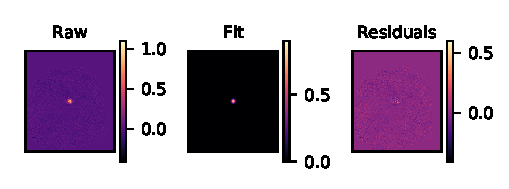
\includegraphics[height=100pt]{CodeAndFigures/DataFits6.pdf}
        \caption{Data:35116}
        \label{fig:lmtFit6}
    \end{subfigure}
    \begin{subfigure}[b]{.45\textwidth}
        \centering
        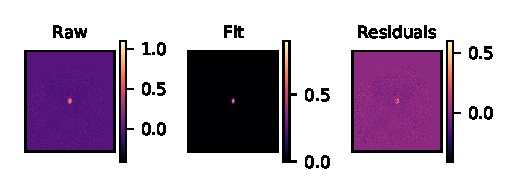
\includegraphics[height=100pt]{CodeAndFigures/DataFits7.pdf}
        \caption{Data:35117}
        \label{fig:lmtFit7}
    \end{subfigure}
    \begin{subfigure}[b]{.45\textwidth}
        \centering
        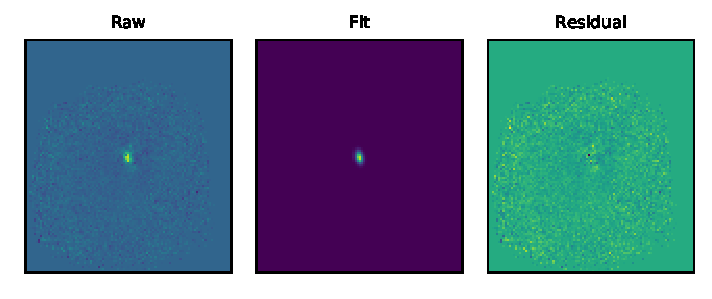
\includegraphics[height=100pt]{CodeAndFigures/DataFits8.pdf}
        \caption{Data:35118}
        \label{fig:lmtFit8}
    \end{subfigure}
    \caption{Image of the raw data, its 2D Gaussian fit and its residuals.}
    \label{fig:lmtRaw}
\end{figure}


\begin{figure}
    \centering
    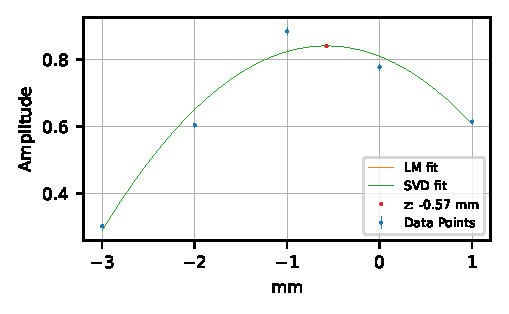
\includegraphics{CodeAndFigures/QuadFitPlot.pdf}
    \caption{Plot of the amplitude obtain by LM method from each maps vs the corresponding z-position of the secondary mirror. }
    \label{fig:lmtquadfit}
\end{figure}

\subsection{}
% Use either the procedure outlined in the class18 notes or the emcee python package to simulate the posterior probability distributions for all of the fitted parameters in one of the 2-d gaussian fits you did. Describe what you see.

We can use a posterior probability distribution of the fitted parameters to estimate the uncertainty in the fit. We start with the best fit parameters from MAP 35116 (Table \ref{tab:lmtMap2}). To do the posterior analysis we do the following
\begin{itemize}
    % \item From our data find the best fit parameters.
    \item Using the best fit parameters simulate N data sets were we randomize new parameters from normal distributions that has the best fit parameters as their mean.
    \item Find the new best fit parameters for the simulated data sets.
\end{itemize}

Figure \ref{fig:lmtpostAna} shows an histogram for each of the parameter and the posterior probability. 

\begin{table}[h]
    \centering
    \begin{tabular}{|c|c|}
        \toprule
         Parameter & Value  \\
         \midrule
         $x_0$       & 154.51 \\
         $y_0$       & 178.55 \\
         $\sigma_x$  & 4.35   \\
         $\sigma_y$  & 4.77   \\
         $\theta$    & 0.59   \\
         Amplitude   & 0.88   \\
         \bottomrule
    \end{tabular}
    \caption{Best fitted parameters from a 2D Gaussian for MAP 35116.}
    \label{tab:lmtMap2}
\end{table}


\begin{figure*}
    \centering
    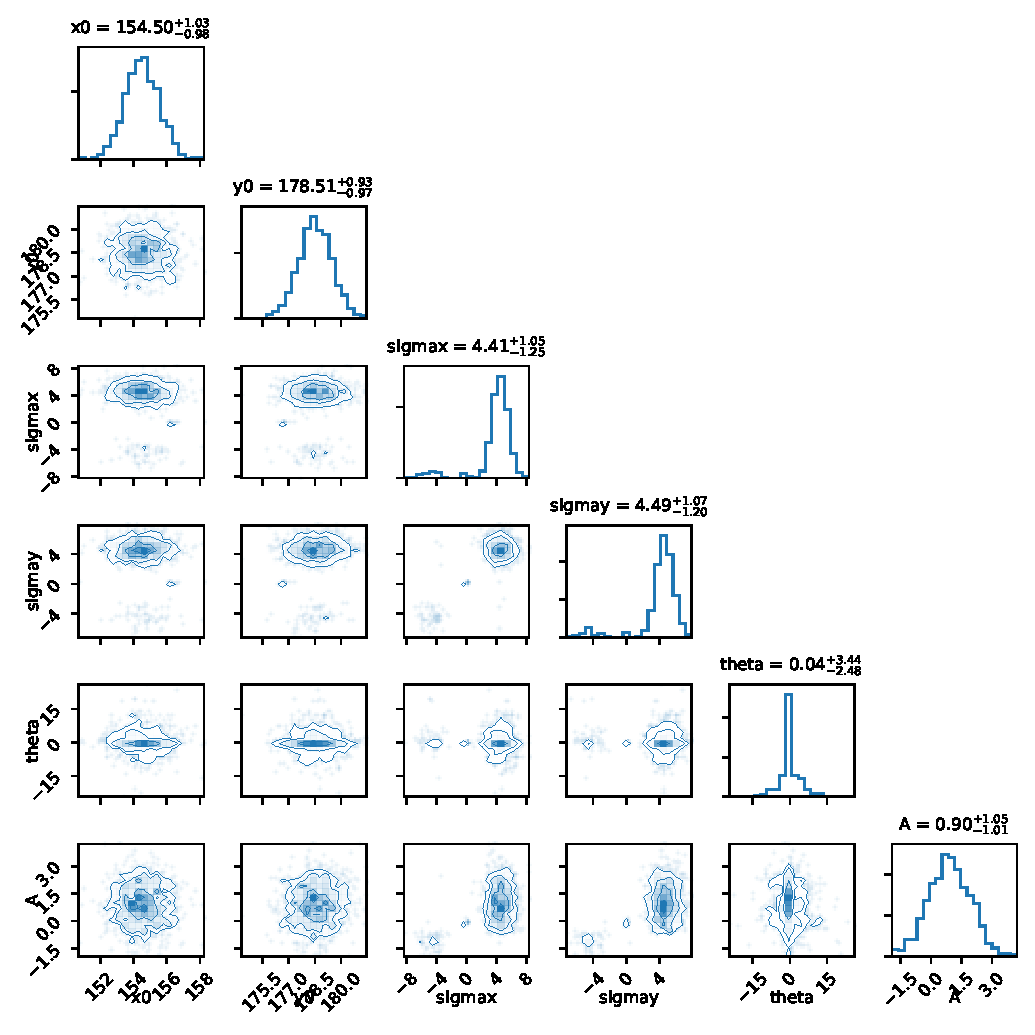
\includegraphics{CodeAndFigures/FocusingLMTPosteriorCorner.pdf}
    \caption{Posterior probability distributions for all of the fitted parameters for MAP 35116.}
    \label{fig:lmtpostAna}
\end{figure*}

